\documentclass{elektr}
\usepackage{amsfonts,amssymb,amsmath,amsgen,amsopn,amsbsy,theorem,graphicx}
\usepackage[utf8]{inputenc}
\usepackage[english]{babel}
\usepackage{multirow,array}
\usepackage[dvipsnames]{xcolor}
\usepackage[pagewise]{lineno}
\linenumbers
\usepackage{float}
\raggedbottom
\usepackage{enumitem}
\setlist{noitemsep, topsep=1pt}
\setlength{\textfloatsep}{6pt plus 1pt minus 2pt}
\setlength{\floatsep}{5pt plus 1pt minus 2pt}
\setlength{\intextsep}{6pt plus 1pt minus 2pt}
\setlength{\abovecaptionskip}{3pt}
\setlength{\belowcaptionskip}{2pt}
\renewcommand{\arraystretch}{0.94}
\usepackage{hyperref}
\hypersetup{colorlinks=true,urlcolor=black,citecolor=blue}




\yil{}
\vol{}
\fpage{}
\lpage{}
\doi{}

\title{QLoRA Fine-Tuning for Consumer Complaint Classification}

\author[Manuscript]{
\rec{}
\acc{}
\finv{}
}
\makeatletter
\gdef\@surnames{Turk J Elec Eng {\&} Comp Sci}
\makeatother

\def\E{\ifmmode{\mathbb E}\else{$\mathbb E$}\fi} %natural numbers
\def\N{\ifmmode{\mathbb N}\else{$\mathbb N$}\fi} %natural numbers
\def\R{\ifmmode{\mathbb R}\else{$\mathbb R$}\fi} %real numbers
\def\Q{\ifmmode{\mathbb Q}\else{$\mathbb Q$}\fi} %rational numbers
\def\C{\ifmmode{\mathbb C}\else{$\mathbb C$}\fi} %complex numbers
\def\H{\ifmmode{\mathbb H}\else{$\mathbb H$}\fi} %complex numbers
\def\Z{\ifmmode{\mathbb Z}\else{$\mathbb Z$}\fi} %integers
\def\P{\ifmmode{\mathbb P}\else{$\mathbb P$}\fi} %real numbers
\def\T{\ifmmode{\mathbb T}\else{$\mathbb T$}\fi} %real numbers
\def\SS{\ifmmode{\mathbb S}\else{$\mathbb S$}\fi} %real numbers
\def\DD{\ifmmode{\mathbb D}\else{$\mathbb D$}\fi} %real numbers

\renewcommand{\a}{\alpha}
\renewcommand{\b}{\beta}
\renewcommand{\d}{\delta}
\newcommand{\D}{\Delta}
\newcommand{\e}{\epsilon}
\newcommand{\var}{\varepsilon}
\newcommand{\g}{\gamma}
\newcommand{\la}{\lambda}
\newcommand{\La}{\Lambda}
\newcommand{\lan}{\langle}
\newcommand{\ran}{\rangle}
\newcommand{\n}{\nabla}
\newcommand{\va}{\varphi}
\newcommand{\s}{\sigma}
\newcommand{\Sig}{\Sigma}
\renewcommand{\t}{\tau}
\renewcommand{\th}{\theta}
\newcommand{\Om}{\Omega}
\newcommand{\om}{\omega}
\newcommand{\pa}{\partial}
\newcommand{\up}{\upsilon}
\newcommand{\vp}{\varphi}
\newcommand{\z}{\zeta}





\newcommand{\bse}{\begin{subequations}}
\newcommand{\ese}{\end{subequations}}
\newcommand{\ben}{\begin{enumerate}}
\newcommand{\een}{\end{enumerate}}
\newcommand{\bens}{\begin{enumerate*}}
\newcommand{\eens}{\end{enumerate*}}
\newcommand{\be}{\begin{equation}}
\newcommand{\ee}{\end{equation}}
\newcommand{\bea}{\begin{eqnarray}}
\newcommand{\eea}{\end{eqnarray}}
\newcommand{\baa}{\begin{eqnarray*}}
\newcommand{\eaa}{\end{eqnarray*}}
\newcommand{\bc}{\begin{center}}
\newcommand{\ec}{\end{center}}
\newcommand{\ol}{\overline}
\newcommand{\ul}{\underline}
\newcommand{\ov}{\overbrace}
\newcommand{\uv}{\underbrace}
\newcommand{\Ra}{\Rightarrow}
\newcommand{\ra}{\rightarrow}
\newcommand{\ds}{\displaystyle}
\newcommand{\vs}{\vspace}


\newcommand{\IR}{\mbox{I \hspace{-0.2cm}R}}
\newcommand{\IN}{\mbox{I \hspace{-0.2cm}N}}



%% \theoremstyle{plain} %% This is the default

\newtheorem{theorem}{Theorem}%[section]

\theoremstyle{corollary}
\newtheorem{corollary}{Corollary}

\theoremstyle{lemma}
\newtheorem{lemma}{Lemma}

\theoremstyle{proposition}
\newtheorem{proposition}{Proposition}

\theoremstyle{axiom}
\newtheorem{axiom}{Axiom}

\theoremstyle{conjecture}
\newtheorem{conjecture}{Conjecture}

\theoremstyle{example}
\newtheorem{example}{Example}

\theoremstyle{definition}
\newtheorem{definition}{Definition}%[section]

\theoremstyle{remark}
\newtheorem{remark}{Remark}%[section]
\newtheorem{notation}{Notation}


\newtheorem{question}{Question}%[section]
\newtheorem{construction}{Construction}

\newtheorem{athm}{Theorem}
\renewcommand{\theathm}{\Alph{athm}}



\setcounter{page}{1}

\setlength{\emergencystretch}{2em}
\begin{document}

\maketitle
\begin{abstract}
We evaluate how QLoRA adaptation changes consumer financial complaint classification under a fixed labelled-data budget. Qwen3-8B and Llama 3.1-8B-Instruct are trained on the same 10,000 examples, with 2,000 validation examples and audited separation from evaluation inputs. On the 15,428-row internal test, three-seed mean macro-F1 rises from 0.6295 to 0.8331 for Qwen and from 0.6247 to 0.8402 for Llama. Paired group-bootstrap gains are 0.2035 [0.1934, 0.2141] and 0.2155 [0.2054, 0.2257]. Both adapted models exceed validation-tuned TF-IDF/Logistic Regression at the matched 10,000-example budget and all three encoder baselines. Full-data TF-IDF reaches 0.8476 using 120,502 training examples. Adaptation substantially improves debt-collection recall, while extending inference text from 500 to 1,500 characters adds 0.0072 and 0.0055 macro-F1 for the adapted models. Controlled batch-one inference adds 0.1224 and 0.0802 seconds per request relative to the corresponding base models. Training-time records and device-specific baseline timings quantify the computational cost alongside these accuracy gains. The results provide an empirical basis for choosing between sparse classification, encoders and adapted generative models according to labelled-data and compute budgets.
\keywords{Consumer complaint classification, large language models, QLoRA, parameter-efficient fine-tuning, model-visible overlap, paired group bootstrap, CFPB}
\end{abstract}

\section{Introduction}
The Consumer Financial Protection Bureau (CFPB) complaint database is a large public corpus of consumer narratives describing financial disputes, product failures, debt collection issues, credit reporting problems, and banking complaints. Accurate classification of such narratives is important for regulatory monitoring, institutional triage, and the prioritisation of consumer-service workflows. The task is challenging because complaint narratives often mention multiple financial products, contain noisy informal descriptions, and must nevertheless be mapped to a single constrained product category.

Recent work has explored large language models (LLMs) for zero-shot complaint classification. In zero-shot settings, models receive the candidate categories in the prompt and must return a valid label without task-specific training. This is attractive for complaint triage because new product taxonomies or institutional routing schemes may be introduced before large labelled datasets are available. However, zero-shot classification also raises practical issues: models can confuse overlapping financial products, output labels outside the allowed taxonomy, and show sensitivity to prompt and deployment details. Once a local zero-shot baseline is established for a given open-weight model, the next methodological question is how much performance can be gained through parameter-efficient fine-tuning under a fixed labelled-data budget.

This paper addresses that question. The central novelty is not a new model architecture or a new fine-tuning algorithm. G\"ull\"u et al. already fine-tuned GPT-2 and Llama 3.1-8B for complaints, including the same five financial categories \cite{gullu2025complaintllm}; Roumeliotis et al. studied zero-shot financial complaint classification \cite{roumeliotis2025think}. Our contribution is a reproducible applied evaluation of the paired zero-shot-to-QLoRA transition, including validation-tuned lighter classifiers and the benefits and costs of adaptation. The primary comparison uses fixed data selections and matched inference settings. Supplementary Section S8 details configuration screening and auxiliary dependence analyses.

The contributions are as follows:
\begin{enumerate}
    \item We compare base zero-shot and QLoRA-adapted models within the same Hugging Face quantised inference pipeline, holding prompt, labels and main input conventions fixed within each model family.
    \item We audit model-visible inputs, quarantine conflicting training/validation records, and preserve evaluation records and the source-related benchmark views with their dependence explicitly accounted for.
    \item We evaluate Qwen3-8B and Llama 3.1-8B across optimisation seeds 42, 43 and 44 on fixed 10,000-example training and 2,000-example validation selections, alongside tuned sparse and encoder baselines.
    \item We report internal and benchmark performance, paired group-bootstrap intervals, separate seed variation, off-label behaviour and class-level error patterns.
    \item We measure same-checkpoint longer-input effects and controlled fresh-call latency to quantify conditional adaptation trade-offs.
\end{enumerate}

\section{Related work}

Classical consumer complaint classification has relied on sparse lexical features, support vector machines, logistic regression, and later transformer encoders. BERT-style models enabled strong supervised text classification by adapting contextual representations to task-specific labels \cite{devlin2019bert}; BERT, DistilBERT, and RoBERTa remain important supervised baselines for complaint categorisation \cite{devlin2019bert,sanh2019distilbert,liu2019roberta,sy2024beyondbert}. Complaint analytics has also been studied across food-industry categorisation, telecom complaint prediction, multicriteria complaint prioritisation, CFPB topic modelling, and financial-complaint interpretability, sentiment, cause, emotion, and severity analysis \cite{bozyigit2022foodcomplaints,gewaly2024telecomcomplaint,vairetti2024complaintpriority,raju2022cfpbtopic,das2024negative}. These studies show that supervised learning can be effective for complaint taxonomies, but they do not directly address how modern open-weight generative models should be adapted and evaluated for the same task.

Recent work has made LLMs relevant to both complaint generation and complaint processing. Large-scale studies report that consumers increasingly use LLMs to draft clearer financial complaints \cite{shin2025adoption,liang2025widespread}, suggesting that complaint corpora are themselves being reshaped by generative AI. LLM-based frameworks have also been investigated for complaint categorisation and customer-service benchmarking \cite{yuan2024framework,li2025teleeval}. Two studies are particularly close to the present work and require separate comparisons.

G\"ull\"u et al. \cite{gullu2025complaintllm} compare CNN, LSTM, BERT, RoBERTa, GPT-2, and Llama 3.1-8B on two datasets: 5,629 Comcast complaints with rating labels and a second dataset reported to contain 162,421 financial complaints in five product categories. The latter categories correspond to the financial taxonomy studied here. Thus, their contribution is not restricted to telecommunications, and the present work cannot be distinguished merely by applying Llama to financial complaints. Their method uses an 80/20 train/test division; Table~V of their paper specifies three training epochs, a 512-token maximum, AdamW, cross-entropy loss, and weighted metric averaging for the LLMs. A LoRA or 4-bit quantisation configuration, a paired zero-shot baseline for each adapted checkpoint, and a three-seed uncertainty summary are not described in that report. Absence of these details is treated as a reporting difference, not evidence that an undocumented procedure was not performed.

Our distinction from G\"ull\"u et al. is the adaptation question and the explicit protocol: 4-bit NF4 LoRA adaptation with completion-only loss for JSON label generation, a fixed 10,000-example training budget, two 8B model families evaluated before and after adaptation in the same inference pipeline, and repeated fine-tuning seeds. Table~\ref{tab:gullu-positioning} summarises these differences. Their published financial-dataset F1 scores should not be ranked against our macro-F1 scores: metric averaging, training budgets, and test construction differ. Nor does their published row count establish exact record-level identity with our 162,415-row source file.

\begin{table}[htbp]
\caption{Protocol comparison with G\"ull\"u et al. \cite{gullu2025complaintllm}. This is a comparison of reported designs, not a cross-paper performance ranking. ``Not described'' refers only to the information available in that paper.}
\label{tab:gullu-positioning}
\begin{center}
\small
\setlength{\tabcolsep}{4pt}
\renewcommand{\arraystretch}{1.12}
\begin{tabular}{@{}>{\raggedright\arraybackslash}p{0.14\linewidth}>{\raggedright\arraybackslash}p{0.40\linewidth}>{\raggedright\arraybackslash}p{0.40\linewidth}@{}}
\hline
\textbf{Aspect} & \textbf{G\"ull\"u et al.} & \textbf{Present study}\\
\hline
Task and data & Comcast rating classification and five-category financial complaints; financial dataset reported as 162,421 records. & Five-category financial complaints from a 162,415-row source file; no new corpus or taxonomy is claimed.\\
Comparison & Supervised comparison of six architectures, including GPT-2 and Llama 3.1-8B. & Paired zero-shot versus QLoRA adaptation for Qwen3-8B and Llama 3.1-8B; TF-IDF and encoders as supervised comparators.\\
Adaptation & LLM training with cross-entropy loss; LoRA and 4-bit settings not described. & Explicit 4-bit NF4 LoRA configuration and completion-only loss for generated JSON labels.\\
Data allocation & 80/20 train/test division; separate validation selection and text-group overlap audits not described. & Model-visible conflicts are quarantined; fixed training/validation selections and evaluation records are retained across all model runs.\\
Budgets & Three LLM epochs and a maximum of 512 tokens. & Two epochs on 10,000 selected training rows per seed; 500 narrative characters within a 512-token prompt budget.\\
Reporting & Accuracy, precision, recall, and weighted F1; three-seed uncertainty summaries not described. & Accuracy, macro-F1, weighted F1, and results across three fine-tuning seeds; separate analysis of adaptation gains.\\
\hline
\end{tabular}
\end{center}
\end{table}

Roumeliotis et al. \cite{roumeliotis2025think} address a different question: zero-shot classification with 14 standard and reasoning LLMs on a balanced 1,000-record CFPB-derived evaluation set. Their preprocessing removes narratives exceeding 500 characters, whereas the present protocol truncates narratives to a maximum of 500 characters and also evaluates the preserved 250/500-character benchmark variants. Their study motivates the five-label JSON-prompt setting, but does not evaluate the paired change caused by task-specific QLoRA adaptation. Our additional model-family and seed comparisons therefore extend the evaluation question rather than claim the first use of this taxonomy or a directly comparable improvement over their published scores.

PEFT provides a middle path between zero-shot inference and full fine-tuning. LoRA learns low-rank adapter matrices while freezing pretrained weights \cite{hu2022lora}, and QLoRA enables quantised LLM adaptation through 4-bit NormalFloat quantisation, double quantisation, and LoRA adapters \cite{dettmers2023qlora}. Other PEFT methods such as prefix tuning and $(IA)^3$ are also viable \cite{li2021prefix,liu2022fewshot}, but QLoRA was selected here for 4-bit adaptation of 8B-class instruction models on 16 GB GPUs. The empirical question is how much same-model adaptation changes classification under the stated budget and how those gains compare with lighter supervised alternatives. It also requires distinguishing source-text grouping from model-visible separation and accounting for overlap among benchmark subsets. These are evaluation requirements for the present study, not claims of a new LoRA or QLoRA algorithm or of the absence of related fine-tuning work.



\section{Materials and methods}
\subsection{Data provenance and preserved evaluation views}
\label{sec:source}
The processed CFPB-related resource is attributed to Tiwari on Kaggle \cite{tiwari2021complaints,cfpbdata}. Its local archive contains 162,421 rows. The working file is identical by index, label and narrative for the first 162,415 rows; six trailing records contain only the placeholder narrative \texttt{name} and are absent. The archive-to-working-file correspondence identifies the analysed source records; the available records do not establish the undocumented preprocessing decisions. Removing ten rows with missing fields leaves 162,405 usable records. Excluding 8,123 benchmark-related source rows leaves a partitioning pool of 154,282 records. The upstream CFPB-to-Kaggle extraction and product-aggregation code is unavailable; source hashes identify the exact analysed input.

The five inherited labels are retail banking, credit reporting, credit card, mortgages and loans, and debt collection. No new upstream product aggregation is performed. Twelve preserved benchmark files contain 1,000 appearances each: sampling-seed identifiers 1/2/3, balanced/imbalanced sampling, and 250/500-character views. Balanced files contain 200 examples per class. Each imbalanced file contains 511 credit-reporting, 182 debt-collection, 107 mortgage/loan, 100 card and 100 banking examples. These files are byte-identical to their source-archive members. The sampling implementation is unavailable; files and construction manifests are supplied. They are source-related benchmark views, not independently collected external data.

\subsection{Model-visible separation and fixed selections}
\label{sec:revised-data}
Data allocation starts from an 80/10/10 split with seed 42 and full-normalised-narrative grouping. Because different full narratives can share a truncated input, label-blind connected components also link normalised 500-character prefixes and reconstructed 512-token inputs. A conservative 250-character prefix guard covers the benchmark views. Evaluation components take priority over fitting records; retained validation components take priority over conflicting training records. Table~\ref{tab:data-flow} reports the resulting exclusions and retained rows.
\begin{table}[htbp]
\caption{Data allocation with model-visible overlap screening. Evaluation records are excluded from fitting.}
\label{tab:data-flow}\centering\small
\begin{tabular}{lrrrr}\hline
Partition & Candidate rows & Excluded & Retained & Groups\\\hline
train & 123427 & 2925 & 120502 & 93609 \\
validation & 15427 & 307 & 15120 & 11925 \\
internal test & 15428 & 0 & 15428 & 12099 \\
\hline

\end{tabular}
\end{table}

Exact-input audits find no shared training/validation-to-evaluation token sequences for the five pinned model tokenizers. Supplementary Section S1 gives the representation checks, audit sizes and longer-input checks; Section S4 describes dependencies among the benchmark views.

One naturally sampled 10,000-row train selection and one 2,000-row validation selection, with selection seed 42, are fixed for every model and optimisation seed. The shared 10k/2k allocation supports matched-data comparisons across model families. Optimisation seeds 42/43/44 change training randomness, not membership. Full-data TF-IDF uses all 120,502 retained training rows. The internal test contains 15,428 rows in 12,099 groups. Evaluation uses a fixed, inspected CFPB-related cohort and is retrospective rather than prospective. Data details and the overlap matrices are in Supplementary Sections S1 and S4.

\subsection{Pinned LLMs, prompting and QLoRA}
\label{sec:llm}
We use Qwen/Qwen3-8B \cite{yang2025qwen3} and meta-llama/Llama-3.1-8B-Instruct \cite{dubey2024llama}. Exact 40-character commits, tokenizer/config files and weight hashes are recorded; Supplementary Section S2 gives the identities. The recorded identities apply to the models in the primary comparison.

Base and adapted models share the same five-label prompt, 500 narrative characters, a 512-token input cap, NF4 4-bit double quantisation and FP16 compute. The 500-character limit holds the paired input convention fixed; 512 is the tokenizer ceiling, not another character limit. Within 500 characters, coverage is 63.98\% among the 162,405 usable source records and 63.01\% in the 154,282-row candidate partitioning pool; these percentages use different populations. Sections~\ref{sec:length-latency} and~\ref{sec:long-results} assess the effects of longer input. The chat template is rendered once and tokenised with \texttt{add\_special\_tokens=False}; Qwen thinking is disabled with \texttt{enable\_thinking=False}. SFT uses the same prompt prefix and completion-only target JSON/EOS; full serialization and target-length checks are detailed in Supplementary Section S2. Greedy generation uses at most 32 new tokens, one beam and no sampling. A regular expression extracts the final \texttt{product} field; absent or invalid labels remain off-label errors. This is JSON prompting with strict parsing, not token-level constrained decoding. No retry, synonym mapping or post-hoc label repair is used.

QLoRA uses rank 16, alpha 32, dropout 0.05 and all-linear targets, with frozen base weights and completion-only cross-entropy. Each fixed-data run has two epochs, learning rate $2\times10^{-4}$, physical batch 1, accumulation 16, paged AdamW 8-bit, cosine scheduling, warmup 0.03 and non-reentrant gradient checkpointing. Validation loss is measured every 100 optimiser steps; the best saved validation-loss checkpoint is retained. These settings are fixed for both LLM families, without test-based configuration selection. Each model has three independently initialised optimisation refits.

The shared configuration is supported by an exploratory Qwen validation comparison of sampling strategy, learning rate, rank and epoch count. Natural sampling, learning rate $2\times10^{-4}$, rank 16 and two epochs have the highest recorded validation macro-F1, 0.8235, among the six screened conditions. Supplementary Section S8 specifies the screening allocation and its limitations. These configuration-screening fits are auxiliary evidence; their validation scores are excluded from the primary test-set comparison. Llama uses the same settings without family-specific optimisation. In contrast, sparse and encoder baselines receive validation searches on the common fitting allocation. The matched-budget comparison therefore includes explicitly tuned baselines rather than relying on extra model-specific QLoRA tuning.

The primary model comparison uses an RTX 5060 Ti 16 GB, driver 595.99.02, Python 3.12.14, PyTorch 2.7.1+cu128 (CUDA 12.8) \cite{paszke2019pytorch}, Transformers 4.57.6 \cite{wolf2020transformers}, PEFT 0.17.1 \cite{mangrulkar2022peft}, TRL 0.23.1, bitsandbytes 0.46.1 and Accelerate 1.10.1. Configuration-screening and auxiliary dependence analyses use the separately documented TRUBA/V100 environment; their scores are excluded from the primary comparison. Each run retains code, versions, manifests and fitted-weight hashes.

\subsection{Validation-tuned supervised baselines}
\label{sec:baselines}
TF-IDF plus Logistic Regression has separate 48-candidate validation searches at the 10k and full-data budgets. Like the neural systems, both sparse budgets use the first 500 narrative characters; the full-data condition increases training rows, not visible text per row. The grid crosses unigram/bigram features, maximum features 50,000/200,000, minimum document frequency 2/5, $C=0.25/1/4$, and no/balanced class weights. Vocabulary/IDF fit training text only. Lowercasing, Unicode accent stripping, sublinear TF and L2 normalisation are fixed. The lbfgs solver uses tolerance $10^{-5}$ and a 2,000-iteration cap; convergence warnings fail the run. Both winners use bigrams, minimum document frequency 5, $C=4$ and no class weighting; feature caps are 50,000 and 200,000. Validation macro-F1 is 0.7989 and 0.8363. Three identical seed-labelled refits at each budget are determinism checks, not stochastic optimisation replicates.

BERT-base-uncased, DistilBERT-base-uncased and RoBERTa-base use all 10k/2k selected rows. Each has six validation candidates: learning rate $2/3/5\times10^{-5}$ crossed with two/three epochs, search seed 42. The maximum final-epoch validation macro-F1 wins; ties within $10^{-12}$ use the smallest predefined candidate ID. Winners are BERT $2\times10^{-5}$/three epochs, DistilBERT and RoBERTa $5\times10^{-5}$/three epochs. Each is freshly refit with seeds 42/43/44 and evaluated at its final epoch. The DistilBERT and RoBERTa selections lie at the upper learning-rate and epoch boundaries of the tested grid; this search does not identify a global optimum. Main encoder inputs are 500 characters with a \textbf{512-token cap}, physical batch 4, accumulation 4, evaluation batch 16, AdamW, weight decay 0.01, linear scheduling, warmup 0.06 and FP16 training/inference. Reloaded predictions must exactly match all 2,000 saved validation predictions before test inference.

A reference-parameter sensitivity uses the encoder token caps and physical batch reported in Tables III--IV of G\"ull\"u et al., with the same selected learning rates and three epochs. Parameter provenance and all six extra refits are in Supplementary Section S7. The primary encoder baselines use 512-token inputs. Our data, 500-character text convention, PyTorch implementation and execution defaults differ from that source, so this is not an exact replication. No baseline is replaced on test performance.

\subsection{Metrics, dependence and uncertainty}
\label{sec:statistics}
The natural CFPB distribution is class-imbalanced, so macro-F1 is emphasised alongside accuracy and weighted F1. Accuracy, macro-F1 and weighted F1 use the same confusion-count estimator. Off-label outputs contribute errors rather than being dropped. Points are observed-data estimates; an adapted system is the mean of three separately scored refits, not an ensemble or a pooled confusion matrix. Run variation is the sample SD ($\mathrm{ddof}=1$). The main and supplementary analyses report stochastic seed SD separately from conditional sampling intervals.

We use 10,000 paired percentile group-bootstrap draws (RNG seed 20261020), sampling whole groups uniformly with replacement. All 19 main prediction variants share the same group multiplicities. Internal metrics retain row weights. Benchmark analysis gives total weight one to each unique (true label, normalised visible narrative) across appearances: 5,909 units in 3,919 conservative full-text/prefix groups. Linked 250/500-character views are sampled together. The twelve overlapping file scores are dependent observations; statistical inference therefore operates on their linked groups. Paired differences are computed within each common resample. Intervals condition on fitted checkpoints and fixed selected configurations; they exclude training/model-selection uncertainty. They are descriptive 95\% intervals without a family-wise multiple-comparison adjustment.

\subsection{Longer inputs and controlled latency}
\label{sec:length-latency}
Each base and adapted checkpoint is evaluated on the same internal IDs under 500 characters/512 tokens, 500/2,048 (a token-cap control), and 1,500/2,048. Training uses 500 characters throughout. The predefined full-narrative $>500$ cohort contains 5,770 rows in 5,131 groups. Input retention and deterministic-response reuse are detailed in Supplementary Sections S2 and S5.

Controlled LLM latency uses fresh batch-one calls on 100 fixed internal IDs (20 per class), ten validation warmups and three repetitions. End-to-end time includes tokenisation, transfer, generation, decoding and parsing; model loading and disk I/O are excluded. CUDA synchronisation and an exclusive GPU-compute check define the timing boundary. Paired intervals use within-ID repetition means. Supplementary Section S6 gives the call-order, precision, output-length and job-block details.

For sparse and encoder baselines, CPU inference uses the same 100 IDs and repetition orders, four CPU threads and fresh calls. Encoders use FP32 and their seed-42 fitted checkpoints; sparse models retain their selected feature maps. Recorded neural training runtimes and fresh fixed-configuration sparse fits provide training wall times. Device and timing boundaries are reported separately so that these implementation costs are not interpreted as a controlled architecture-only speed comparison.

\section{Results}
\subsection{Model comparison}
\label{sec:main-results}
Table~\ref{tab:models} combines the fixed-data LLMs, tuned encoders and sparse baselines. Qwen macro-F1 rises from 0.6295 to 0.8331 and Llama from 0.6247 to 0.8402. Seed SD is 0.0048/0.0020 for the adapted models. Their paired macro-F1 gains are 0.2035 [0.1934, 0.2141] and 0.2155 [0.2054, 0.2257], conditional on these fitted checkpoints.
\begin{table}[H]
\caption{Internal test (15,428 rows). Macro-F1 brackets are 95\% paired-group intervals; SD is across three actual optimisation refits. Base systems have no adaptation rows. TF-IDF SD zero denotes deterministic checks. Full-data TF-IDF has a larger training budget.}
\label{tab:models}\centering\small\renewcommand{\arraystretch}{1.08}\setlength{\tabcolsep}{3pt}
\begin{tabular}{@{}lrrrrr@{}}\hline
System & Train rows & Macro-F1 [CI] & Seed SD & Accuracy & Weighted F1\\\hline
Qwen3 base & 0 & 0.6295 [0.6182, 0.6405] & --- & 0.7352 & 0.7206 \\
Qwen3 QLoRA & 10,000 & 0.8331 [0.8245, 0.8411] & 0.0048 & 0.8689 & 0.8678 \\
Llama 3.1 base & 0 & 0.6247 [0.6138, 0.6349] & --- & 0.7295 & 0.7177 \\
Llama 3.1 QLoRA & 10,000 & 0.8402 [0.8312, 0.8483] & 0.0020 & 0.8736 & 0.8729 \\
BERT & 10,000 & 0.8119 [0.8028, 0.8203] & 0.0010 & 0.8541 & 0.8528 \\
DistilBERT & 10,000 & 0.8104 [0.8014, 0.8188] & 0.0065 & 0.8522 & 0.8511 \\
RoBERTa & 10,000 & 0.8105 [0.8015, 0.8187] & 0.0039 & 0.8525 & 0.8520 \\
TF-IDF/LR 10k & 10,000 & 0.8068 [0.7973, 0.8157] & 0.0000 & 0.8499 & 0.8474 \\
TF-IDF/LR full & 120,502 & 0.8476 [0.8402, 0.8549] & 0.0000 & 0.8805 & 0.8798 \\
\hline

\end{tabular}
\end{table}

At the matched 10k budget, QLoRA exceeds TF-IDF macro-F1 by 0.0263 and 0.0334, with paired intervals above zero (Table~\ref{tab:contrasts}). Encoder differences from the sparse baseline are smaller, with macro-F1 intervals spanning zero. Full-data TF-IDF reaches 0.8476; Qwen's difference from it is $-0.0145$, whereas Llama's $-0.0074$ interval includes zero (unrounded upper bound $6.8\times10^{-6}$). Direct matched-budget encoder contrasts are also positive: Qwen QLoRA exceeds the three encoders by 0.0212--0.0227 macro-F1 and Llama by 0.0283--0.0297; all six paired intervals exclude zero (Table~\ref{tab:contrasts}). The consolidated points and intervals share one estimator; bootstrap means are not substituted for observed points.
\begin{table}[H]
\caption{Internal macro-F1 paired differences, comparison minus reference. All intervals condition on fitted models. Rows using full-data TF-IDF provide unequal-training-budget context.}
\label{tab:contrasts}\centering\small\renewcommand{\arraystretch}{1.08}
\begin{tabular}{llrr}\hline
Reference & Comparison & Difference & 95\% CI\\\hline
Qwen3 base & Qwen3 QLoRA & 0.2035 & [0.1934, 0.2141] \\
Llama 3.1 base & Llama 3.1 QLoRA & 0.2155 & [0.2054, 0.2257] \\
TF-IDF/LR 10k & Qwen3 QLoRA & 0.0263 & [0.0199, 0.0327] \\
TF-IDF/LR 10k & Llama 3.1 QLoRA & 0.0334 & [0.0270, 0.0397] \\
TF-IDF/LR 10k & BERT & 0.0051 & [-0.0013, 0.0117] \\
TF-IDF/LR 10k & DistilBERT & 0.0036 & [-0.0025, 0.0098] \\
TF-IDF/LR 10k & RoBERTa & 0.0037 & [-0.0025, 0.0098] \\
TF-IDF/LR full & Qwen3 QLoRA & -0.0145 & [-0.0221, -0.0071] \\
TF-IDF/LR full & Llama 3.1 QLoRA & -0.0074 & [-0.0153, 0.0000] \\
\hline

\end{tabular}
\end{table}

\subsection{Benchmark views, classes and output compliance}
\label{sec:legacy-errors}
Unique-input-weighted benchmark macro-F1 is 0.6324/0.8210 for base/adapted Qwen and 0.6271/0.8272 for Llama. Paired gains are 0.1886 [0.1723, 0.2051] and 0.2000 [0.1838, 0.2166]. Matched-budget TF-IDF gives 0.7871; full-data TF-IDF gives 0.8347. The overlapping views support a dependence-aware source-related analysis, not twelve independent replications or external generalisation. Supplementary Sections S3--S4 give all metrics, seeds and per-view descriptions.

Figure~\ref{fig:corrected-confusion} and the supplementary class tables describe the primary-comparison predictions. Debt-collection recall rises from 0.3262 to 0.7347 for Qwen and from 0.2754 to 0.7540 for Llama. Improvements are not uniform: Qwen credit-card recall changes from 0.7637 to 0.7550 despite its higher class F1. Of 15,428 internal predictions, Qwen base has one off-label output and each adapted refit has zero; Llama base and each refit have one. These are observed compliance counts, not enforced constrained decoding or evidence of prompt robustness. Residual confusions and different class supports remain important.

The dominant zero-shot error is the confusion of \texttt{debt\_collection} with \texttt{credit\_reporting}. Qwen makes this error 1,232 times before adaptation and 430.33 times after adaptation on average; the corresponding Llama counts are 1,167 and 403.33. These are reductions of 65.1\% and 65.4\%. Fine-tuning also reduces \texttt{retail\_banking} $\rightarrow$ \texttt{credit\_card} errors from 562 to 81 for Qwen and from 263 to 89 for Llama. Adapted counts are means of three refit count matrices; fractional values do not denote fractional complaints in a single run.

One residual issue remains visible in both models: \texttt{credit\_reporting} $\rightarrow$ \texttt{debt\_collection} errors increase from 142 to 344 for Qwen and from 87 to 336 for Llama. Higher debt-collection recall therefore coexists with more false assignments from the majority class. The main change is a redistribution of errors across neighbouring financial categories, rather than a uniform improvement in every decision boundary. These descriptive counts locate the remaining problem; they do not establish its causal mechanism or the operational cost of particular mistakes.
\begin{figure}[htbp]\centering
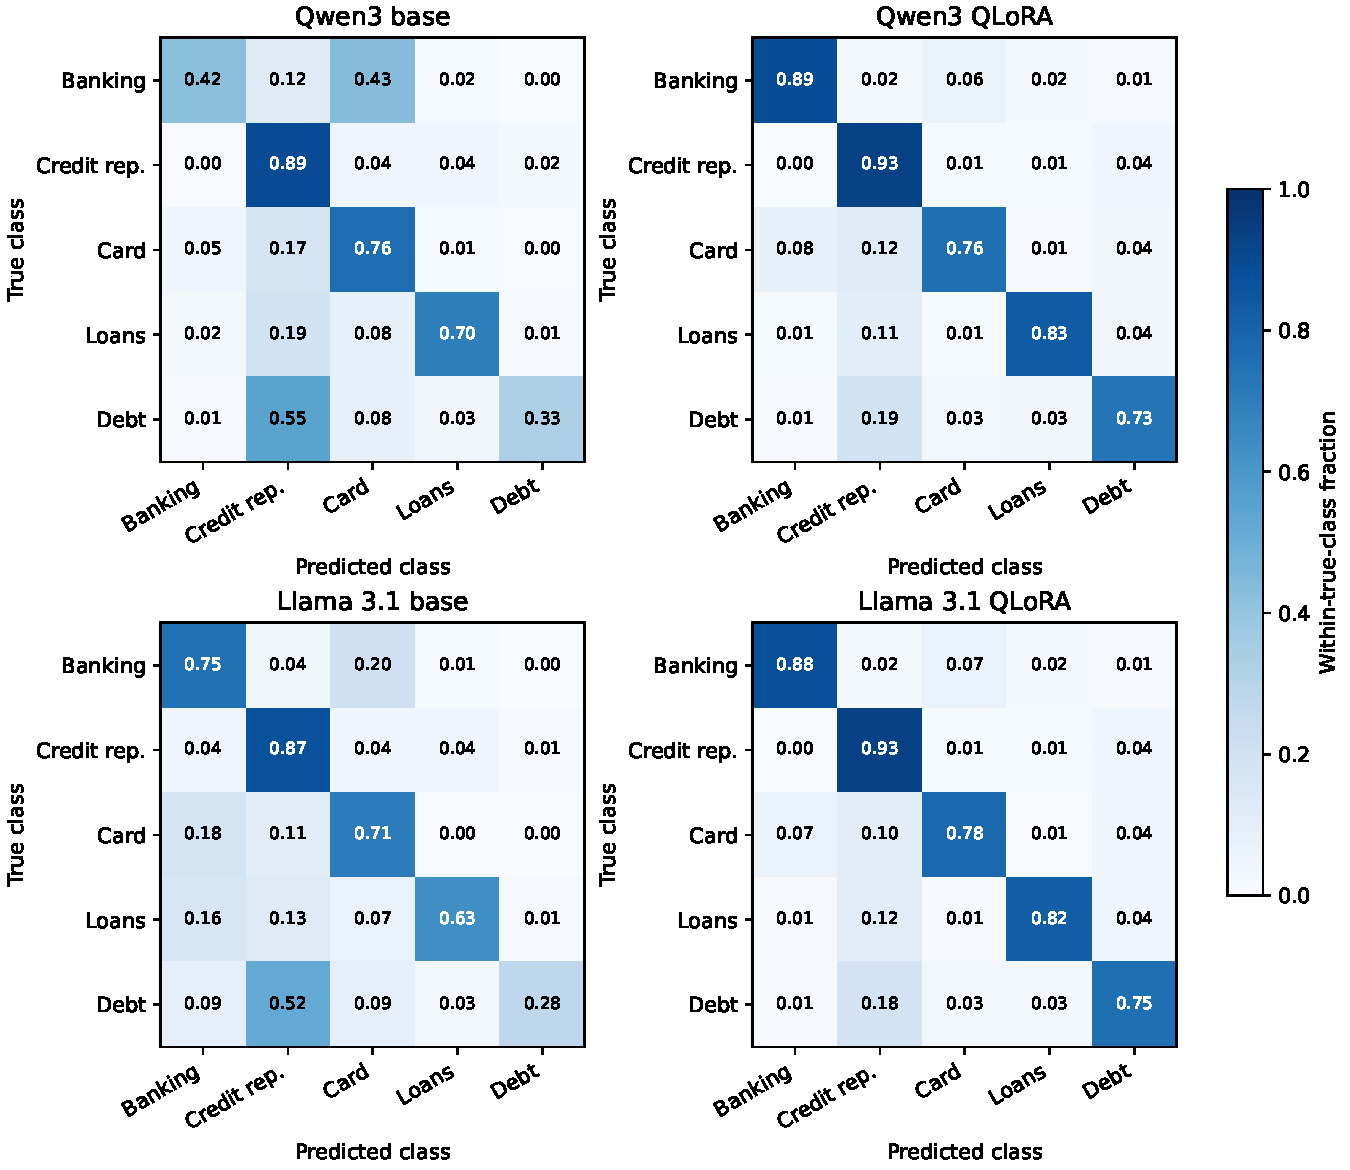
\includegraphics[width=0.90\linewidth]{figures/corrected_confusion_matrices.pdf}
\caption{Internal confusion fractions, normalised within true class. QLoRA matrices average the three refit count matrices before normalisation; performance metrics are means of separately scored runs. Class order and off-label counts are supplied in Supplementary Section S3.}
\label{fig:corrected-confusion}
\end{figure}

\subsection{Same-checkpoint longer-input results}
\label{sec:long-results}
The 500/512 and 500/2,048 control predictions are identical. Increasing visible text to 1,500 characters improves adapted Qwen/Llama macro-F1 by 0.0072/0.0055 overall and by 0.0156/0.0117 in the longer-narrative cohort (Table~\ref{tab:long}). Zero-shot Qwen instead declines; the zero-shot Llama interval includes zero. The result supports a conditional benefit of longer input for these adapted checkpoints, not a universal improvement or an evaluation of longer-context training. Supplementary Section S5 also reports auxiliary length-stratum descriptions and matched 250/500-character benchmark views; their cohort and fitting conditions differ from this controlled inference comparison.
\begin{table}[htbp]
\caption{Macro-F1 change for 1,500 versus 500 characters, both with a 2,048-token cap. ``All'' includes 15,428 rows; $>500$ is the predefined 5,770-row cohort. QLoRA is the three-seed mean.}
\label{tab:long}\centering\small\renewcommand{\arraystretch}{1.08}\setlength{\tabcolsep}{3pt}
\begin{tabular}{lllrrrr}\hline
Model & Variant & Cohort & 500 & 1,500 & Difference & 95\% CI\\\hline
Qwen3 & base & All & 0.6295 & 0.6224 & -0.0072 & [-0.0107, -0.0036] \\
Qwen3 & QLoRA mean & All & 0.8331 & 0.8403 & 0.0072 & [0.0048, 0.0097] \\
Qwen3 & base & $>500$ & 0.6316 & 0.6135 & -0.0181 & [-0.0262, -0.0099] \\
Qwen3 & QLoRA mean & $>500$ & 0.8484 & 0.8640 & 0.0156 & [0.0105, 0.0209] \\
Llama 3.1 & base & All & 0.6247 & 0.6227 & -0.0020 & [-0.0058, 0.0018] \\
Llama 3.1 & QLoRA mean & All & 0.8402 & 0.8456 & 0.0055 & [0.0029, 0.0081] \\
Llama 3.1 & base & $>500$ & 0.6432 & 0.6415 & -0.0017 & [-0.0102, 0.0068] \\
Llama 3.1 & QLoRA mean & $>500$ & 0.8562 & 0.8679 & 0.0117 & [0.0065, 0.0172] \\
\hline

\end{tabular}
\end{table}

\subsection{Controlled inference cost and supplementary sensitivity}
\label{sec:cost-results}
For 500/512, mean end-to-end seconds are 0.2896/0.4120 for base/adapted Qwen and 0.2831/0.3633 for Llama (Table~\ref{tab:latency}). The additional mean times are 0.1224 [0.1166, 0.1284] and 0.0802 [0.0758, 0.0847]. These differences include actual generated lengths and adapter execution, not an isolated adapter-overhead experiment. The balanced 100-record cohort and serial batch-one calls are not an operational workload benchmark. Full per-seed median/p95, token counts and all conditions are in Supplementary Section S6.
\begin{table}[htbp]
\caption{Fresh-call end-to-end latency (seconds), 500 characters/512 tokens, RTX 5060 Ti. QLoRA mean averages the three variant means; paired intervals use within-ID repetition means.}
\label{tab:latency}\centering\small
\begin{tabular}{lrrrr}\hline
Model & Base mean & QLoRA mean & Added time & 95\% CI\\\hline
Qwen3 & 0.2896 & 0.4120 & 0.1224 & [0.1166, 0.1284] \\
Llama 3.1 & 0.2831 & 0.3633 & 0.0802 & [0.0758, 0.0847] \\
\hline

\end{tabular}
\end{table}

Table~\ref{tab:compute-cost} places these LLM timings alongside the measured CPU baselines and training wall times. The sparse models provide the lowest compute-cost option in these implementations. Encoder inference occupies an intermediate range on the CPU; adapted LLM inference uses the GPU. Supplementary Section S8 gives per-method fitting/search times, CPU median/p95 latency and measurement scopes.
\begin{table}[htbp]
\caption{Implementation-specific compute costs. Neural fitting uses the RTX 5060 Ti; sparse fitting and baseline inference use a four-thread CPU. Fit times are per refit; LLM inference is NF4/FP16 on GPU and encoder inference is FP32 on CPU. Device differences preclude architecture-only speed claims.}
\label{tab:compute-cost}\centering\small
\begin{tabular}{lrrrr}\hline
System & Fit min & Fit device & E2E ms & Inference device\\\hline
Qwen3 QLoRA & 417.67 & GPU & 411.98 & GPU \\
Llama 3.1 QLoRA & 429.25 & GPU & 363.28 & GPU \\
BERT & 2.56 & GPU & 39.68 & CPU \\
DistilBERT & 1.53 & GPU & 19.51 & CPU \\
RoBERTa & 2.72 & GPU & 35.82 & CPU \\
TF-IDF/LR 10k & 0.03 & CPU & 0.38 & CPU \\
TF-IDF/LR full & 0.80 & CPU & 0.29 & CPU \\
\hline

\end{tabular}
\end{table}

The separately declared Ref [14] conditions give internal macro-F1 0.8102 for BERT and 0.8095 for RoBERTa versus main values 0.8119/0.8105. Paired difference intervals span zero. The main RoBERTa condition uses 512 tokens. All source-specific parameter differences and three refits are reported in Supplementary Section S7 without selecting a replacement on test performance.

\section{Discussion}
\label{sec:discussion}
At the matched 10,000-example budget, QLoRA provides clear gains over each model's zero-shot baseline, validation-tuned sparse classification and all three encoder baselines. Llama QLoRA reaches macro-F1 0.8402 with 10,000 labelled training examples, compared with 0.8476 for TF-IDF trained on 120,502 examples: about one twelfth as many training labels. Its paired difference is $-0.0074$, with an interval spanning zero (unrounded upper bound $+6.8\times10^{-6}$). This is compatible with a small performance difference, rather than evidence of statistical equivalence or non-inferiority. The label-budget result must be weighed against the substantially greater fitting and inference cost of the LLMs. Where labels and compute are both available, full-data sparse classification remains a strong practical choice.

Model-visible separation is central to the comparison because full-text duplicate detection alone does not identify all collisions under truncation. Grouping the visible representations and excluding fitting conflicts provides an explicit basis for the paired evaluation. The auxiliary dependence analyses in Supplementary Sections S5 and S8 quantify the limitations of full-text grouping; their different memberships, model identities and environments preclude attributing cross-condition score differences solely to overlap handling.

The class-level pattern is particularly relevant for complaint triage. Debt collection narratives may mention disputed accounts, credit bureaus and credit reports, so the five-label task has closely related categories. The reduction in debt-to-reporting errors is accompanied by increased reporting-to-debt errors, which helps explain why a gain in aggregate macro-F1 does not resolve every routing concern. The balanced benchmark views expose minority-class behaviour, while the imbalanced views retain different class prevalences; their overlap requires the shared-group analysis rather than treating them as independent confirmations. Human review, cost-sensitive training and class-specific calibration are possible directions for studying these residual errors, not evaluated safeguards in the present experiments.

Related work already establishes complaint LLM fine-tuning. Our distinction from G\"ull\"u et al. is the explicit NF4/LoRA and completion-only protocol, paired same-model baseline, fixed adaptation membership and separated uncertainty; from Roumeliotis et al., it is the adaptation comparison beyond zero-shot evaluation. Different splits, metrics and budgets preclude cross-paper performance ranking. Longer input helps the adapted checkpoints here, while zero-shot results show that more text alone is not a general solution. Latency intervals quantify conditional measured costs; their operational acceptability requires workload-specific evidence.

\section{Limitations}
\label{sec:limitations}
Evaluation is retrospective on previously inspected CFPB-related records; there is no independent-source, temporal or prospective generalisation test. Exact-input audits and conservative groups do not eliminate semantic duplication. Bootstrap intervals condition on fixed refits and the chosen protocol, excluding training/model-selection uncertainty. Three seeds give limited evidence about training variation, and multiple intervals are not family-wise adjusted. The 10k budget, fixed prompt and two 8B model families do not establish an optimal sample size, prompt robustness or universal classifier ranking.

The longer-input comparison changes inference text only; the models were trained with at most 500 characters. Latency uses serial unmerged-adapter jobs, a balanced 100-record sample and separate variant blocks, leaving thermal/background drift and output-length effects. CPU baseline and GPU LLM timings describe different implementations and precision settings; thermal/background drift can remain. Training wall times have method-specific validation/preprocessing boundaries, and encoder search totals cover training phases rather than full wall time. Energy, concurrent service capacity and total hardware lifecycle cost are not measured. Upstream CFPB-to-Kaggle preprocessing is unavailable. Some auxiliary fits also lack complete fitted weights and immutable upstream identities, limiting their reconstruction; Supplementary Section S8 states this scope separately from the fully identified primary models.

\section{Conclusion}
\label{sec:conclusion}
QLoRA raises internal macro-F1 by about 0.20 for two 8B model families under a fixed 10,000-example training budget. Both adapted models outperform the matched-data sparse and encoder baselines, and substantially improve debt-collection recall. The adapters also benefit from longer inference text despite being trained with 500-character inputs. Llama QLoRA approaches the observed full-data sparse score using about one twelfth of its training labels, at a higher computational cost. Together, the matched-data comparisons, class-level results and measured costs support a practical choice: sparse classifiers offer an efficient default, while QLoRA can provide stronger fixed-budget classification when an adapted generative model fits the intended workflow.
\section*{Acknowledgment and/or disclaimers, if any}
The authors acknowledge the TRUBA ARF infrastructure operated by T\"UB\.{I}TAK ULAKB\.{I}M for computational resources supporting configuration screening and auxiliary analyses. The primary model comparison uses a local RTX 5060 Ti 16 GB.

\section*{Declaration of Generative AI and AI-assisted technologies, if any}
AI-assisted tools supported analysis-code preparation, literature comparison, wording and LaTeX formatting. Numerical results come from recorded computations and independently checked prediction files. The authors retain responsibility for source verification, interpretation, final review and the submitted manuscript.

\section*{Data availability statement}
The source data derive from the CFPB complaint database and the processed Kaggle resource attributed to Tiwari \cite{cfpbdata,tiwari2021complaints}. Source/derived data, fixed selections, code, configurations, model identities, validation and final predictions, and statistical evidence are provided in the reproducibility repository at \url{https://github.com/muhammettan28/CFPB_tuning}. Supplementary Section S8 describes its contents and the CPU result-verification procedure. The repository excludes third-party literature and neural-model weights. Limitations concerning upstream preprocessing and auxiliary-model reconstruction are documented in Supplementary Section S8.

\section*{Funding, if any}
The authors received no specific funding for this study.
\section*{Conflict of interest, if any}
The authors declare no conflict of interest.

\begin{thebibliography}{99}
\setlength{\itemsep}{1pt}
\setlength{\parsep}{0pt}

\bibitem{devlin2019bert} Devlin J, Chang MW, Lee K, Toutanova K. BERT: pre-training of deep bidirectional transformers for language understanding. In: Proceedings of NAACL-HLT; Minneapolis, MN, USA; 2019. pp. 4171-4186.

\bibitem{sanh2019distilbert} Sanh V, Debut L, Chaumond J, Wolf T. DistilBERT, a distilled version of BERT: smaller, faster, cheaper and lighter. arXiv:1910.01108, 2019.

\bibitem{liu2019roberta} Liu Y, Ott M, Goyal N, Du J, Joshi M et al. RoBERTa: a robustly optimized BERT pretraining approach. arXiv:1907.11692, 2019.

\bibitem{sy2024beyondbert} Sy CY, Maceda LL, Canon MJP, Flores NM. Beyond BERT: exploring the efficacy of RoBERTa and ALBERT in supervised multiclass text classification. International Journal of Advanced Computer Science and Applications 2024; 15 (3). doi: 10.14569/IJACSA.2024.0150323.

\bibitem{bozyigit2022foodcomplaints} Bozyiğit F, Doğan O, Kılınç D. Categorization of customer complaints in food industry using machine learning approaches. Journal of Intelligent Systems: Theory and Applications 2022; 5 (1): 85-91. doi: 10.38016/jista.954098.

\bibitem{gewaly2024telecomcomplaint} Gewaly MM, Saeed MS, Ammar AM. Machine learning approach for complaint prediction in the telecom industry. In: 2024 Intelligent Methods, Systems, and Applications; 2024. pp. 12-17. doi: 10.1109/IMSA61967.2024.10652677.

\bibitem{vairetti2024complaintpriority} Vairetti C, Aránguiz I, Maldonado S, Karmy JP, Leal A. Analytics-driven complaint prioritisation via deep learning and multicriteria decision-making. European Journal of Operational Research 2024; 312 (3): 1108-1118.

\bibitem{raju2022cfpbtopic} Sangaraju VR, Bolla BK, Nayak DK, Kh J. Topic modelling on Consumer Financial Protection Bureau data: an approach using BERT based embeddings. arXiv:2205.07259, 2022.

\bibitem{das2024negative} Das S, Singh A, Saha S, Maurya A. Negative review or complaint? Exploring interpretability in financial complaints. IEEE Transactions on Computational Social Systems 2024; 11 (3): 3606-3615. doi: 10.1109/TCSS.2023.3338357.

\bibitem{shin2025adoption} Shin M, Kim J, Shin J. The adoption and efficacy of large language models: evidence from consumer complaints in the financial industry. arXiv:2311.16466, 2025.

\bibitem{liang2025widespread} Liang W, Zhang Y, Codreanu M, Wang J, Cao H et al. The widespread adoption of large language model-assisted writing across society. arXiv:2502.09747, 2025.

\bibitem{yuan2024framework} Yuan L, Ouyang X, Bai R, Zhu X, Zhou Y et al. A framework for categorizing complaint text via large language model. In: 2024 7th International Conference on Advanced Algorithms and Control Engineering; 2024. pp. 519-523. doi: 10.1109/ICAACE61206.2024.10549750.

\bibitem{li2025teleeval} Li F, Wang Y, Xu Y, Wang S, Liang J et al. Performance evaluations of large language models for customer service. International Journal of Machine Learning and Cybernetics 2025; 16: 2997-3017. doi: 10.1007/s13042-024-02432-9.

\bibitem{gullu2025complaintllm} Güllü M, Atagün E, Biroğul S, Barışçı N. Customer complaint classification with large language models. In: 2025 International Conference on Artificial Intelligence, Computer, Data Sciences and Applications; Antalya, Türkiye; 2025. pp. 1-6. doi: 10.1109/ACDSA65407.2025.11166338.

\bibitem{roumeliotis2025think} Roumeliotis KI, Tselikas ND, Nasiopoulos DK. Think before you classify: the rise of reasoning large language models for consumer complaint detection and classification. Electronics 2025; 14: 1070. doi: 10.3390/electronics14061070.

\bibitem{hu2022lora} Hu EJ, Shen Y, Wallis P, Allen-Zhu Z, Li Y et al. LoRA: low-rank adaptation of large language models. In: International Conference on Learning Representations; 2022.

\bibitem{dettmers2023qlora} Dettmers T, Pagnoni A, Holtzman A, Zettlemoyer L. QLoRA: efficient finetuning of quantized LLMs. In: Advances in Neural Information Processing Systems; 2023.

\bibitem{li2021prefix} Li XL, Liang P. Prefix-tuning: optimizing continuous prompts for generation. In: Proceedings of ACL-IJCNLP; 2021. pp. 4582-4597.

\bibitem{liu2022fewshot} Liu H, Tam D, Muqeeth M, Mohta J, Huang T et al. Few-shot parameter-efficient fine-tuning is better and cheaper than in-context learning. In: Advances in Neural Information Processing Systems; 2022.

\bibitem{cfpbdata} Consumer Financial Protection Bureau. Consumer complaint database. Website https://www.consumerfinance.gov/data-research/consumer-complaints/ [accessed 01 July 2026].

\bibitem{yang2025qwen3} Yang A, Li A, Yang B, Zhang B, Hui B et al. Qwen3 technical report. arXiv:2505.09388, 2025.

\bibitem{dubey2024llama} Grattafiori A, Dubey A, Jauhri A, Pandey A, Kadian A et al. The Llama 3 herd of models. arXiv:2407.21783, 2024.

\bibitem{paszke2019pytorch} Paszke A, Gross S, Massa F, Lerer A, Bradbury J et al. PyTorch: an imperative style, high-performance deep learning library. In: Advances in Neural Information Processing Systems; 2019. pp. 8024-8035.

\bibitem{wolf2020transformers} Wolf T, Debut L, Sanh V, Chaumond J, Delangue C et al. Transformers: state-of-the-art natural language processing. In: Proceedings of EMNLP: System Demonstrations; Online; 2020. pp. 38-45.

\bibitem{mangrulkar2022peft} Mangrulkar S, Gugger S, Debut L, Belkada Y, Paul S et al. PEFT: state-of-the-art parameter-efficient fine-tuning methods. GitHub repository, 2022.

\bibitem{tiwari2021complaints} Tiwari S. Consumer complaints dataset for NLP. Kaggle, 2021. Website https://www.kaggle.com/datasets/shashwatwork/consume-complaints-dataset-fo-nlp [project archive].

\end{thebibliography}


\end{document}
